\section{Results}

All numbers in this section are outputs of the model described above, including the assumptions in
Table~\ref{tab:struct}. We emphasize the relative effects of the measures; the absolute minutes and percentages are
illustrative.

The main experiments use $p_{occ}=0.4$ (about 570 elevator riders per changeover), $q=0.6$, and $a=0.2$.
We chose $p_{occ}$ so that the baseline reproduces the qualitative description of a long line before every
class without collapse; this is a calibration to a description, not a validation (Table~\ref{tab:struct}).
Section~\ref{sec:occ} shows how the results change with occupancy.

\subsection{Behavioral measures}

\begin{table}[h]
\centering
\caption{Policies without an offset ($o=0$). Wait is mean $\pm$ standard error across replicates; late is the
share of students arriving after class start. Absolute values are illustrative outputs of the model.}
\label{tab:policy}
\begin{tabular}{lrrrrr}
\toprule
Policy & Mean wait (s) & P90 wait (min) & Late (\%) & Empty stops (\%) & Clear (min)\\
\midrule
Baseline   & $314 \pm 8$ & 12.4 & $22.9 \pm 1.4$ & 14.5 & 25.0\\
Backpacks  & $217 \pm 6$ &  8.7 & $12.7 \pm 1.2$ &  9.3 & 20.2\\
Walking    & $294 \pm 8$ & 11.9 & $19.6 \pm 1.3$ & 13.9 & 24.6\\
Both       & $203 \pm 6$ &  8.5 & $11.0 \pm 1.0$ &  8.7 & 19.9\\
\bottomrule
\end{tabular}
\end{table}

Table~\ref{tab:policy} and Figure~\ref{fig:wait} show the headline result. Holding backpacks in front reduces
mean wait by 31\% and nearly halves the share of late students. Walking is much weaker: it removes only about
7\% of elevator riders, because floors 2 and~3 hold 9 of the 54 rooms and only partial compliance is
realistic on the way up. Together the two measures reduce mean wait by 35\%, to 3.4 minutes, and lateness
from 22.9\% to 11.0\%. The effect of backpacks is nearly linear in compliance: each additional 25\% of
compliance removes roughly 20--30 seconds of mean wait (Figure~\ref{fig:comp}). Part of this linearity is built in,
because compliance enters the model as a per-car probability of two extra seats; see Section~\ref{sec:struct}.

\begin{figure}[h]
\centering
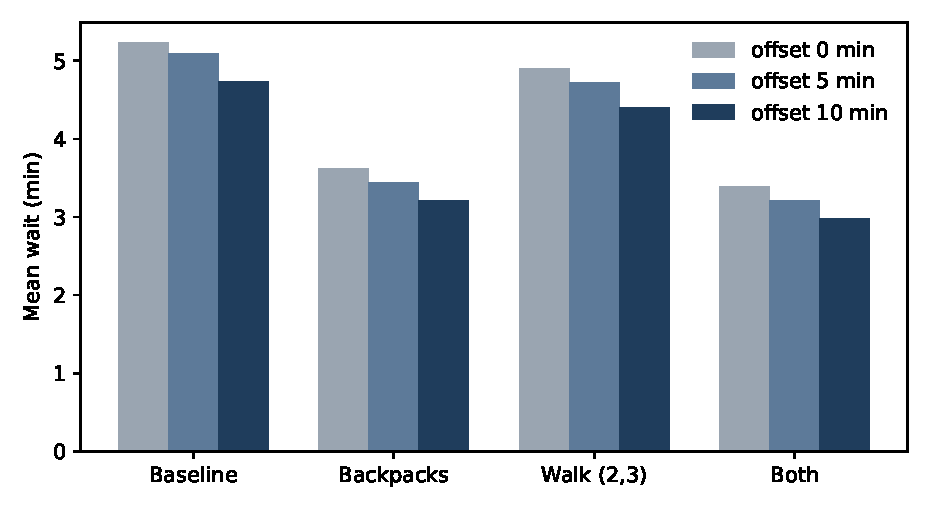
\includegraphics[width=0.8\linewidth]{fig_wait_policy_offset.pdf}
\caption{Mean wait by policy and offset of floors 10--14.}
\label{fig:wait}
\end{figure}

\begin{figure}[h]
\centering
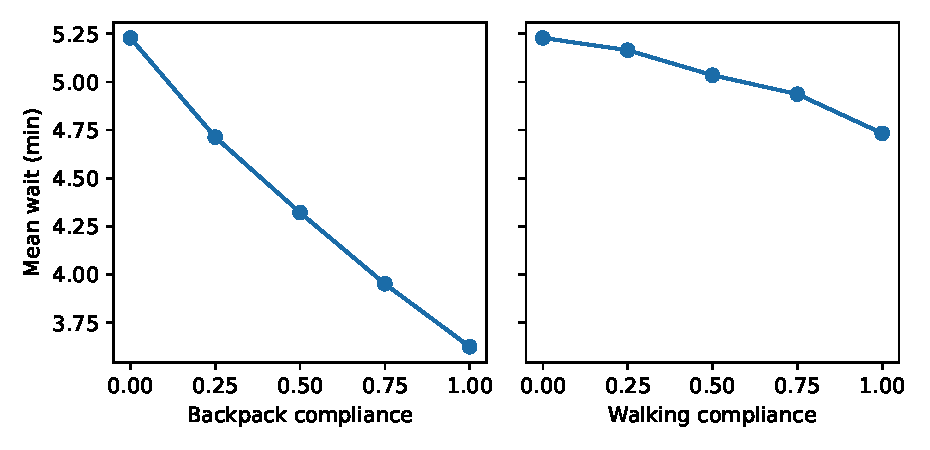
\includegraphics[width=0.8\linewidth]{fig_compliance.pdf}
\caption{Mean wait as compliance grows. Left: backpacks. Right: walking (down-compliance shown; up-compliance
scaled at 0.6 and 0.25 for floors 2 and 3).}
\label{fig:comp}
\end{figure}

Figure~\ref{fig:queue} shows why. Immediately after class ends, about 300 people are waiting in the baseline
and the queue drains slowly; the arriving students then add to a backlog that has not cleared when the
next class starts. The combined measures lower the peak and, more importantly, speed up the drain.

\begin{figure}[h]
\centering
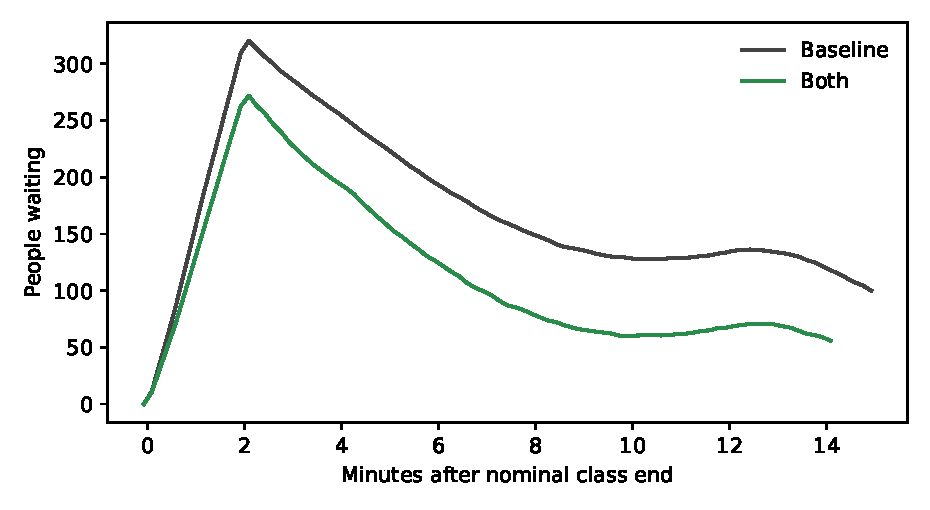
\includegraphics[width=0.8\linewidth]{fig_queue_series.pdf}
\caption{People waiting for an elevator over the passing period (mean of replicates, $o=0$).}
\label{fig:queue}
\end{figure}

\subsection{Where the waiting happens}

Waits are not uniform across the building (Figure~\ref{fig:floor}). Floor~10, the first floor served only by the
two-car bank, is the worst: riders there wait about 10 minutes in the baseline and 7.5 minutes with both
measures. Floors 5--7 are next, at about 5--6 minutes. The measures help everywhere but do not remove the upper-floor
bottleneck, which comes from the structure of the banks.

\begin{figure}[h]
\centering
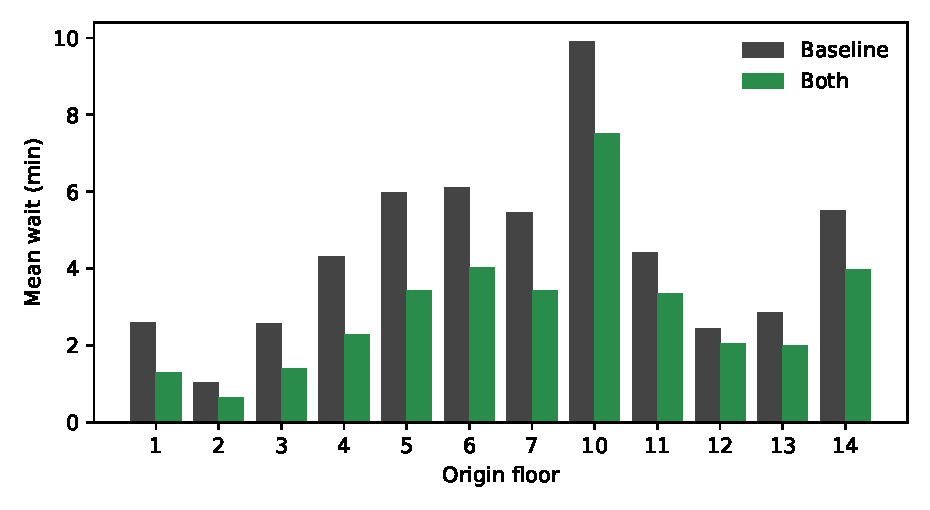
\includegraphics[width=0.8\linewidth]{fig_wait_by_floor.pdf}
\caption{Mean wait by origin floor, baseline versus both measures ($o=0$).}
\label{fig:floor}
\end{figure}

\subsection{Time-multiplexing the upper floors}

\begin{table}[h]
\centering
\caption{Effect of running floors 10--14 $o$ minutes early.}
\label{tab:offset}
\begin{tabular}{lrrrr}
\toprule
Policy & Offset (min) & Mean wait (s) & Late (\%) & Clear (min)\\
\midrule
Baseline & 0  & 314 & 22.9 & 25.0\\
Baseline & 5  & 305 & 24.2 & 22.3\\
Baseline & 10 & 284 & 23.2 & 19.5\\
Both     & 0  & 203 & 11.0 & 19.9\\
Both     & 5  & 192 & 12.5 & 17.5\\
Both     & 10 & 179 & 14.4 & 15.9\\
\bottomrule
\end{tabular}
\end{table}

These offset results are preliminary: a single changeover cannot capture how a shifted clock affects transfers
across the whole teaching day (Section~\ref{sec:future}, item~6).
An offset trades one problem for another (Table~\ref{tab:offset}, Figures~\ref{fig:wait} and~\ref{fig:late}).
A 10-minute offset shortens the mean wait by about 9\% in the baseline and 12\% with both measures, and shortens
the time to clear the queue by 22\% and 20\%. It does not reduce lateness: in the baseline the change is within
noise, and with both measures lateness \emph{increases} from 11.0\% to 14.4\%, because students moving from a
lower floor to an upper one now have only five minutes. Students moving between adjacent floors are
unaffected, since the group boundary falls between floors 7 and 10, which have no classrooms in between;
the cost falls entirely on students changing between the lower and upper groups. A 5-minute offset gives
about half of the reduction in clearing time at about half of the added lateness, so we regard it as the more defensible choice if the
registrar would consider off-grid start times.

\begin{figure}[h]
\centering
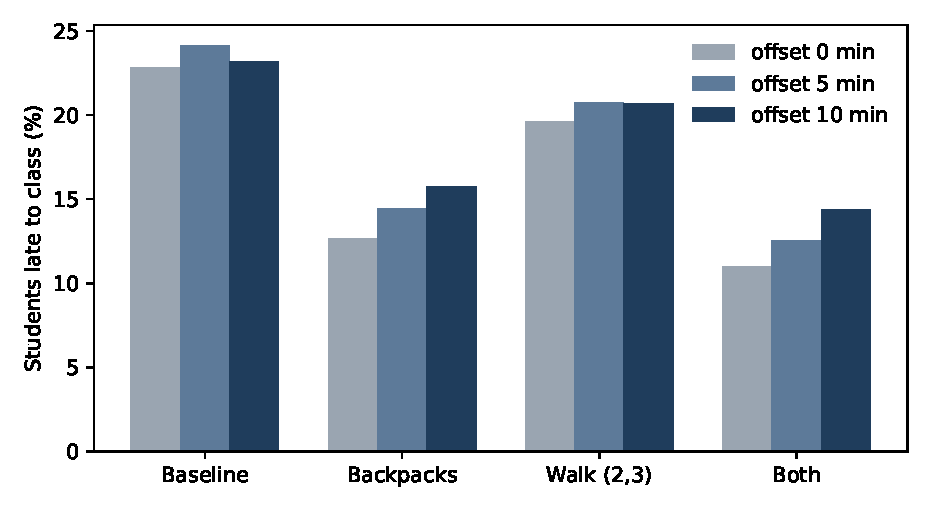
\includegraphics[width=0.8\linewidth]{fig_late_policy_offset.pdf}
\caption{Share of students arriving after class start, by policy and offset.}
\label{fig:late}
\end{figure}

\subsection{Sensitivity to parameters}
\label{sec:occ}

The sweeps below vary parameters only. The structural assumptions of Table~\ref{tab:struct} are the same in every
run.

\paragraph{Occupancy.} The absolute waits depend strongly on how many rooms are in use
(Figure~\ref{fig:occ}): from 2.6 minutes at 20\% occupancy to 17 minutes at full occupancy in the baseline.
The relative benefit of backpacks plus walking is stable, between 29\% and 36\% across the whole range.
At 20\% occupancy the baseline already has 7.9\% late students, rising to 62\% at full occupancy.

\begin{figure}[h]
\centering
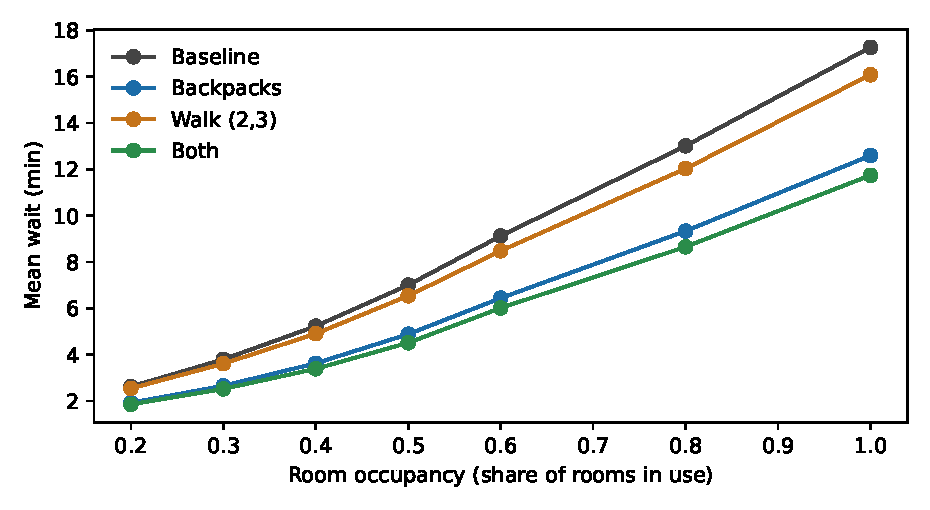
\includegraphics[width=0.8\linewidth]{fig_occupancy_sweep.pdf}
\caption{Mean wait as room occupancy grows.}
\label{fig:occ}
\end{figure}

\paragraph{Door time.} Doubling the door time per stop from 5 to 12 seconds raises the baseline mean wait from 236
to 432 seconds, while the relative benefit of both measures stays between 34\% and 36\%. Door time matters
because every empty stop costs a full door cycle; this is the direct cost of the lack of a full-car bypass.

\paragraph{Adjacent-floor transfers.} Varying the share of transfers that go to an adjacent floor from 10\% to 30\%
changes the late share by only 1--2.5 points in either direction (Figure~\ref{fig:adj}), because without stairs the
adjacent-floor riders still use the elevators. Offering stairs for one-floor trips, an extension beyond the
two measures requested, reduces the combined-policy mean wait from 196 to 176 seconds
(about 10\%) at an adjacent share of 30\% and 80\% stair use, and the late share from 10.4\% to 9.1\%.

\begin{figure}[h]
\centering
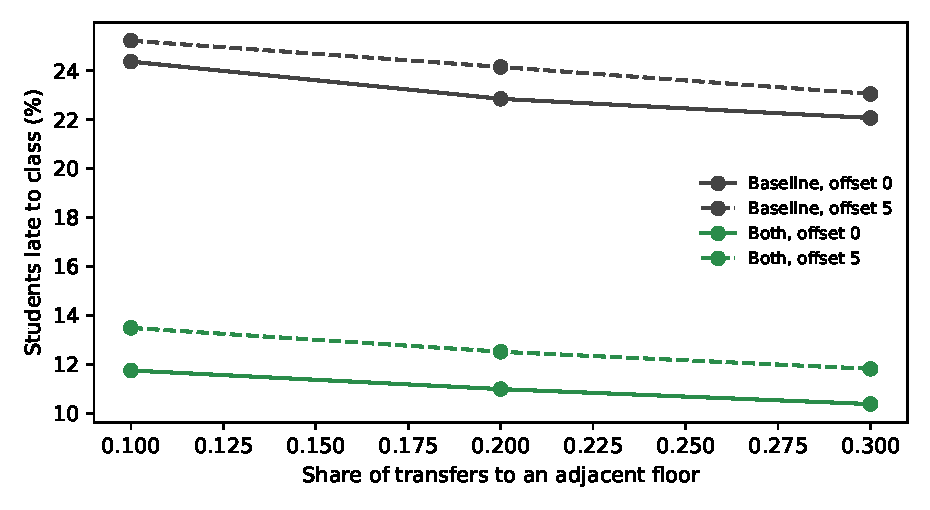
\includegraphics[width=0.8\linewidth]{fig_adjacent_share.pdf}
\caption{Share of late students against the adjacent-floor share of transfers.}
\label{fig:adj}
\end{figure}
